\documentclass[12pt]{article}

\usepackage{sbc-template}

\usepackage{graphicx,url}

%\usepackage[brazil]{babel}   
\usepackage[utf8]{inputenc}  

     
\sloppy

\title{Implementação de Rede Corporativa pela Empresa Shelby Network no Supermercado NeoMart Carpina-PE}

\author{Davi Barbosa\inst{1}, Gabriel Correia (Gerente)\inst{2}, Lucas Mateus\inst{3} Vinícius Mateus\inst{4}}

\address{Curso Técnico em Redes de Computadores --\\ Escola Técnica Maria Eduarda Ramos de Barros
  (ETEMERB)\\
  Caixa Postal 15.064 -- 91.501-970 -- Porto Alegre -- RS -- Brazil
\nextinstitute
  Curso Técnico em Redes de Computadores\\
  Escola Técnica Maria Eduarda Ramos de Barros 
  \email{\{nedel,flavio\}@inf.ufrgs.br, R.Bordini@durham.ac.uk,
  jomi@inf.furb.br}
}

\begin{document} 

\maketitle

\begin{abstract}
  The objective of the proposed project, from the structuring and implementation of a computer network inside a enterprise that planning to implement your supermarket chain in Carpina-PE town, makes own planning be influenced to choice good products and services for the specific supermarket aim, from all the management of the employers to the internal sensitive generated data security and the physical machines placed in the local. Into the workflow of the project, the topics elements will discuss pass by pass of this implementation, e.g the networking addressing, topology, choice operating systems, in-use services and the user control inside all machines and as well the backup strategy planning, with the focus in helper all those who will use these technologies.
\end{abstract}
     
\begin{resumo} 
  O objetivo do projeto proposto, da estruturação e implementação de uma rede de computadores numa empresa que tem por objetivo implantar sua rede de supermercados na zona rural no município de Carpina-PE, tenciona nosso planejamento para escolhermos bons produtos e serviços para a finalidade específica de um supermercado, desde todo o gerenciamento dos funcionários a segurança interna dos dados e das máquinas físicas disposta no local. Ao decorrer do projeto, os elementos dos tópicos irão destrinchar parte a parte dessa implementação, discutindo a rede de forma física e lógica, como por exemplo o endereçamento, topologia, sistemas escolhidos, softwares em uso e o controle de usuários nas máquinas e assim como o planejamento do backup, com o foco de ajudar todos aqueles que irão utilizar essas tecnologias.
\end{resumo}

\section{Introdução}
 A revolução tecnológica chegou pra ficar e prosperar ainda mais, ano após ano, as empresas observam e concluem que sem a Internet não há meios cabíveis de realizar a troca e a comunicação de forma segura com e priorizando as partes envolvidas, e diante da demanda da necessidade de controlar grandes quantias de informações, é de extrema importância e necessidade de possuímos uma rede de computadores de forma estruturada ao qual garanta a comunicação das máquinas prestando a usabilidade, praticidade e segurança na execução das atividades dentro dos setores de um estabelecimento. Nós da Shelby Network vamos ao longo deste projeto implementar por formas práticas e meios cabíveis, uma rede de computadores estruturada para uma rede de supermercado conhecida como NeoMart que deseja implantar sua empresa na região de Carpina-PE, configurando e adaptando os dispositivos na rede as necessidade dos clientes e funcionários da mesma, suprindo assim a demanda do consumidor.

\section{Shelby Network}
Nossa empresa, a Shelby Network, tem como objetivo fornecer dispositivos e infraestrutura de TI com a melhor qualidade, eficiência na entrega e disponibilidade dos produtos e da construção ao controle dos dispositivos dentro da rede. Somos a inovação no mercado buscando sempre garantir além de bons produtos e uma ótima infraestrutura de rede que possibilite uma fácil configuração (a desejar do cliente) adaptando as necessidades de cada setor, a funcionalidade plena de todos os setores atendidos e ajudando assim a sua empresa a crescer com os nossos serviços.

\begin{figure}[ht]
\centering

\includegraphics[height=0.4\textwidth]{logo.PNG}
\caption{Logo da Empresa Shelby}
\label{fig:adds-pastas}
\end{figure}

\section{Objetivos}

\subsection{Geral}
Implementar uma rede de computadores num supermercado dentro do município de Carpina-PE, a empresa em questão denominada de NeoMart, deseja trazer sua rede de supermercados para a região.

\subsection{Específicos}
Planejamento da rede lógica: criar e consolidar uma topologia de rede lógica que garanta a rapidez e o não interrompimento dos serviços disponibilizados pelo supermercado, suprindo ao mesmo tempo a segurança dos dados internos gerados pela empresa.
Planejamento da rede física: escolher bons produtos para que os funcionários, clientes de nossa infraestrutura, sejam beneficiados pelos serviços e de tal modo aumentar sua produtividade.
Escolha de serviços: A parte usual, sensível para os usuários e para empresa, a escolha dos softwares e serviços é essencial para cumprir com as necessidades do supermercado.
Criação de políticas: Diversas políticas são necessárias nesse âmbito do trabalho, como políticas de senha, acesso ao servidor e etc.
Criação do planejamento central: Vários planejamentos para a implementação são necessários, como o controle de usuário dentro da rede através das políticas de grupo.
Planejamento da redundância: Itens como provedores de Internet, Backup dos dados gerados pelo supermercado tem que receber sua devida atenção durante o planejamento da redundância dentre as vias implementadas.

\section{Justificativa}
Diante das necessidades atuais por inovações na área tecnologia, é de extrema importância aderir a um sistema computadorizado, ao qual permite o acesso rápido e fácil para desde da manipulação, a conservação dos dados geridos pelos vários funcionários da empresa. Essa tecnologia de compartilhamento se dá pela redes de computadores, que se tornou algo extremamente essencial no mundo atual, a facilidade que essa tecnologia juntamente com a quantidade de serviços disponibilizados por ela tornou simples e eficaz a comunicação e a resolução de possíveis problemas que, como por exemplo, o supermercado em questão vier a ter e necessitar. Nós da Shelby Network propomos com esse projeto estruturar e configurar os meios responsáveis para que haja um padrão e a qualidade da infraestrutura que foi nos proposto resolver, assim, criando um projeto ao qual garanta a disponibilidade das necessidades do setor do supermercado à segurança dos dados sensíveis do mesmo.

\section{Lista de Keywords}
WI-FI - Wireless Fidelity
TI/IT - Information Technology
SSH - Secure Shell
ADDS - Active Directory Domain Server
DNS - Domain Name Server
RAM - Random Access Memory
PC - Personal Computers
OS - Operating System
Mbps - Megabits per second
VM - Virtual Machine
DHCP - Dynamic Host Configuration Protocol
HD - Hard Disk
GPO - Group Policy Objects
VPN - Virtual Private Network

\section{Sistemas Operacionais e Serviços da Rede}

\subsection{Visão por cima}
Utilizaremos o Windows 10 Pro para os funcionários que irão atender os caixas, setores administrativos integrando também o SAC e com o sistema Debian GNU/Linux versão 11 e Windows Server para os servidores, compondo assim o ambiente integrado de TI. A justificativa da escolha dos sistemas operacionais são esclarecidas abaixo.

\subsection{Serviços Disponibilizados na Rede}
Selecionamos os melhores serviços para fornecer a melhor experiência dentro da rede do supermercado. Segue a lista dos serviços escolhidos e o esclarecimento do porque os escolhemos.

\begin{center}
\begin{tabular}{| l | r | r | r | r |}
\hline
Serviço & Identificador & Disponibilidade & Local de Execução\\
\hline
Antivírus & 2 & Local & Windows Server + Clientes\\
ADDS & 11 & Local & Windows Server\\
Servidor de Arquivos & 4 & Local & Windows Server\\
SSH & 6 & Local & Debian GNU/Linux\\
DNS & 7 & Local & Debian GNU/Linux\\
Samba & 9 & Local & Debian GNU/Linux\\
Servidor Web e Proxy & 10 & Local & Debian GNU/Linux\\
VPN & 3 & Externa & MikroTik\\
DHCP & 8 & Local & MikroTik\\
Armazenamento em Nuvem & 5 & Local & -\\
Firewall & 1 & Local & Todas as Máquinas\\
Hotspot & 12 & Local & -\\
\hline
\end{tabular}
\end{center}

\subsection{Windows 10 Pro}
Optado por fornecer tecnologias em que a integridade de dados da empresa prevalece com o sistemas BitLocker na qual criptografa os recursos presentes nos HD(s), assim protegendo as informações dos usuários. Mensuramos também a capacidade de se aplicar as políticas de grupos, que nos apresentar uma forma de tratar e gerenciar regras definidas para máquinas ou grupos de usuários, utilizaremos esse controle em nossa infraestrutura.

\subsubsection{Antivírus em Execução}
O serviço de antivírus que utilizaremos é o Norton, este serviço possui um console e será gerenciado pelo servidor, além de está em plena execução em todas as máquinas dos funcionários ao qual executam o sistema Windows, o objetivo da implementação é garantir uma melhor utilização dos recursos das máquinas, a supervisão sobre as máquinas, a proteção real oferecida pela solução e a capacidade de agendar o fluxo de verificação analítica (que decorre mais tempo e é de extrema importância a não interrupção dos funcionários em tempo de serviço). O plano de verificação analítica propõem o gerenciamento deste fluxo.

\subsection{Windows Server Essential e Seus Serviços}
Irá possuir e fornecer o serviço do Active Directory (ADDS), podendo assim, gerenciar todas as máquinas e clientes envolvidos dentro da rede interna com a ajuda do servidor Debian suprindo as demais funcionalidades e serviços.

\subsubsection{ADDS}
O Active Directory é onde será implementado informações de acesso sobre os usuários, incluindo os usuários e computadores existentes, definindo também as permissões de cada usuário dentro do sistema. Através dele será verificado o fator da autenticidade, ou seja, se a pessoa realmente é quem ela afirma ser.\newline 
Através do AD, somos capazes de distinguir os grupos perante a suas atividades exercidas dentro da empresa. Por exemplo, podemos definir uma regra básica que ajude aos funcionários do setor do caixa (pertencente ao grupo "Caixas") a executar automaticamente o software de gestão empresarial, possibilitando aos funcionários com poucos cliques “Inicializar a sua área de trabalho”, além da capacidade de mover a área de trabalho de cada usuário nos computadores que fornecem aquele mesma classe de função.


\subsubsection{Controle de Usuários}
O controle de usuários, realizado no ADDS, nos beneficia desde a criação a administração destes usuários. Os usuários ficaram dispostos em sua unidade organizacional que obedece o seu setor em específico, cada unidade organizacional possui um grupo ao qual possui todos os usuários da unidade em específica, possibilitando de uma maneira mais fácil gerir as permissões destes usuários. Abaixo, um exemplo de como isso funcionará:

\begin{figure}[ht]
\centering
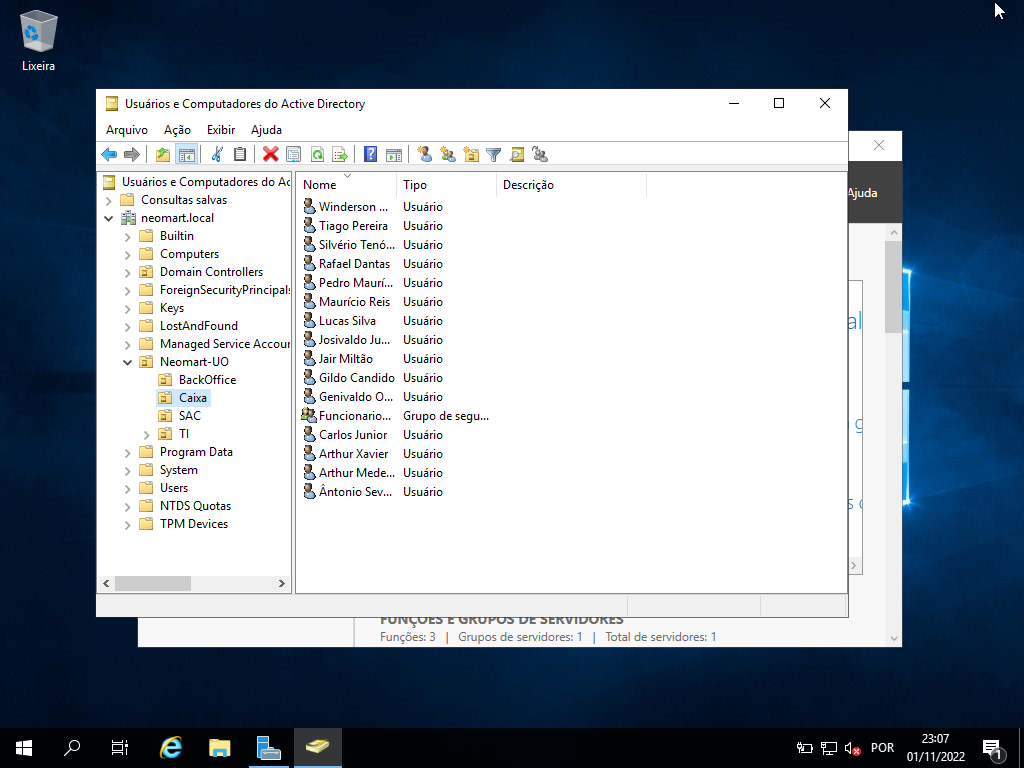
\includegraphics[height=0.5\textwidth]{adds-unidades-usuarios.png}
\caption{Grupos de usuários no ADDS}
\label{fig:adds-pastas}
\end{figure}

\subsubsection{Implementação do GPO}
O Group Policy (GPO), políticas de grupo ou diretivas de grupo, é através deste recurso que vamos configurar as políticas de cada grupo de usuários dentro do nosso domínio. As configurações ficarão de acordo com a necessidade dos setores:

\begin{center}
\begin{tabular}{| l | r | r | r |}
\hline
Setor & Permissões (Nível de Privilégios)\\
\hline
TI & 0\\
BackOffice & 1\\
SAC & 1\\
Caixa & 2\\ 
\hline
\end{tabular}
\end{center}

\begin{enumerate}
    \item Nível 0: Pode realizar qualquer modificação a nível de administrador das máquinas dentro dos demais setores.
    \item Nível 1: É proibido a instalação/remoção de programas dentro das máquinas. É proibido a alteração das configurações de redes dos computadores.
    \item Nível 2: É proibido o poder de gravação do usuário em mídias graváveis, como por exemplo (Pendrive, Cartão de memória; HD/SSD); É proibido alterar o plano de fundo da máquina. - INCLUI TODAS AS RESTRIÇÕES DO NÍVEL 1.
\end{enumerate}

\subsubsection{Demonstração da Implementação das Políticas de Grupo}

\begin{figure}[ht]
\centering
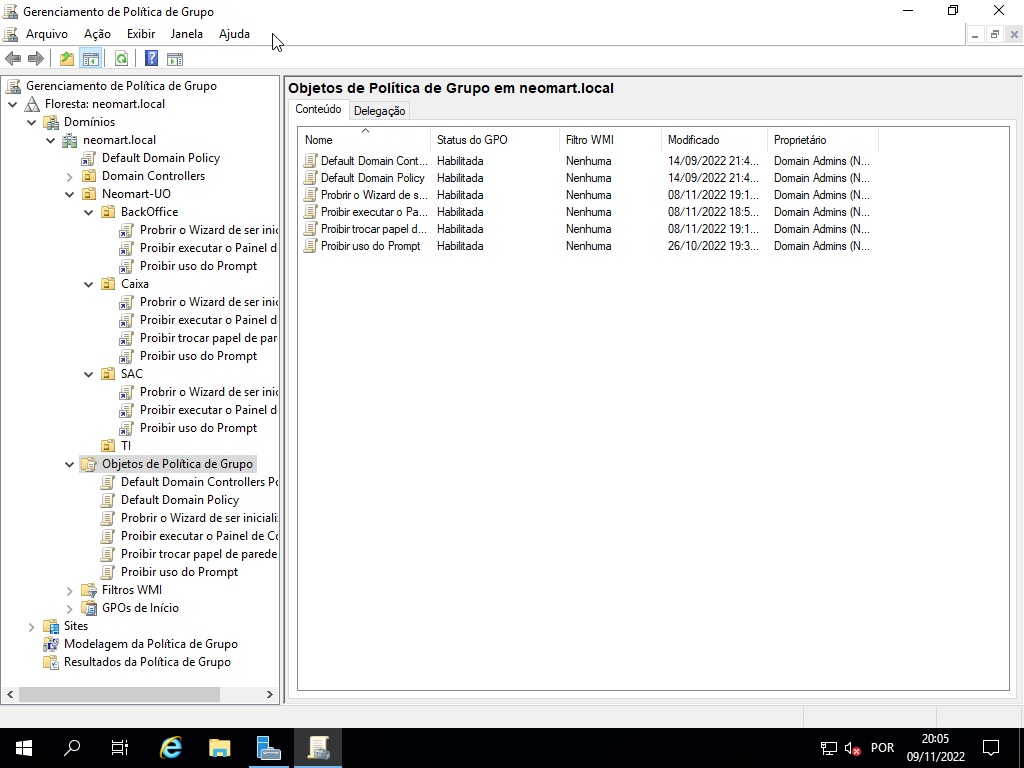
\includegraphics[height=0.5\textwidth]{adds-regras.png}
\caption{Regras do controle de usuários no ADDS}
\label{fig:adds-pastas}
\end{figure}

\subsubsection{Servidor de Arquivos}
Criamos diretórios no caminho \textbf{“C:/Funcionarios”} no servidor que contém o ADDS (Windows Server) em execução, com o nome de cada setor e através da ferramenta chamada “Gerenciador de Recursos de Servidor de Arquivos” adicionamos as entradas para cada setor com regras de cotas de armazenamento aplicadas de maneira permissivas, possibilitando até mais de 100GB de armazenamento para todos os setores.

\begin{figure}[ht]
\centering
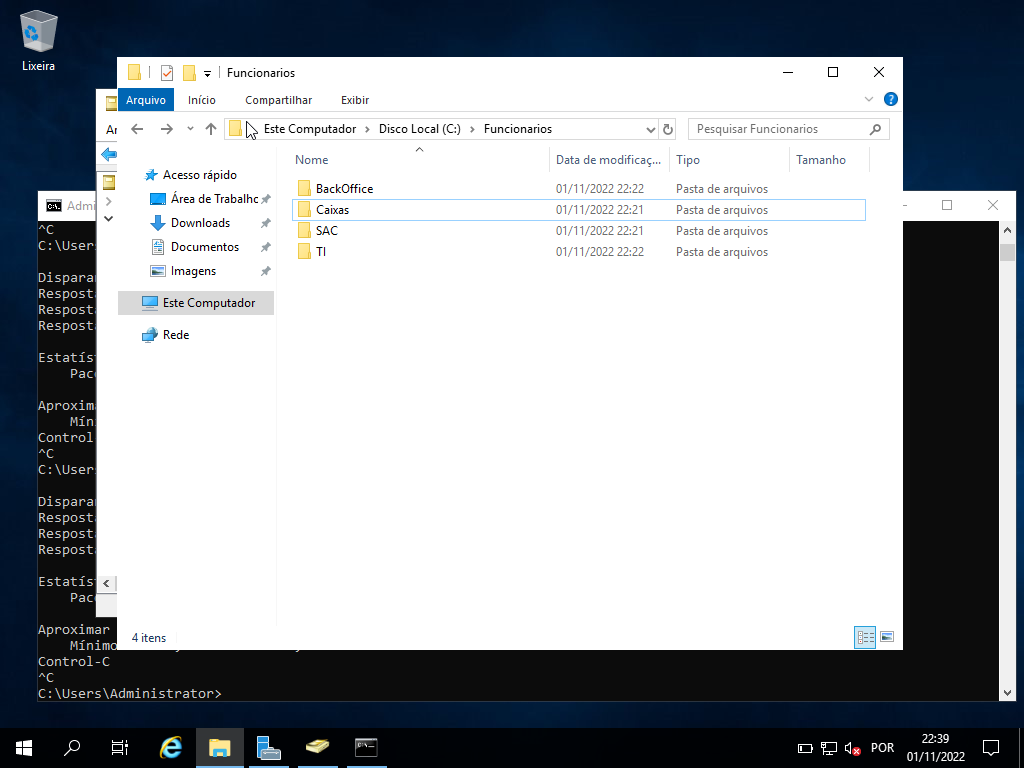
\includegraphics[height=0.5\textwidth]{adds-pasta-compartilhada.png}
\caption{Estrutura de diretórios no servidor ADDS}
\label{fig:adds-pastas}
\end{figure}

\newpage

\subsection{Debian Server GNU/Linux e Seus Serviços}
Com a tecnologia oferecida pela comunidade do Debian, os demais clientes e o servidor Windows Server irão se beneficiar dos serviços oferecidos pelo servidor previamente configurado, fornecendo assim os serviços de DNS; SSH e o SAMBA, esse por sua vez possibilitando a comunicação entre as máquinas Windows com o GNU/Linux.

\subsubsection{SSH}
Para a utilização remota do servidor Debian, utilizaremos o openssh para realizar a comunicação de maneira segura e autêntica, garantindo a confiabilidade e o registro (log) do acesso dos administradores ao servidor Linux. Serviço disponibilizado na porta 22 com autenticação por senha e proibição ao usuário root por motivos de segurança.

\subsubsection{DNS}
Utilizaremos um serviço privado de DNS dentro da nossa infraestrutura para possibilitar o controle dentre as máquinas dos setores e juntamente com os serviços e impressoras em rede estáticas, podendo assim visualizar e administrar os recursos dentro da nossa rede. Utilizaremos o software bind9 no Debian GNU/Linux para suprir as necessidades.

\subsubsection{Samba}
O Samba é um serviço utilizado através do GNU/Linux em conjunto ao ADDS, possibilitando o controle e o uso integrados de ambos os serviços. A partir dele poderemos controlar o ADDS através do SSH, o Samba será executado no mesmo servidor onde o DNS está sendo executado, o Debian.

\subsubsection{Web e Proxy}
Para o servidor de Proxy, utilizaremos o serviço squid no servidor Debian GNU/Linux, através dessa ferramenta seremos capazes de manipular o nó de saída da comunicação interna da rede. O squid trabalha com os seguintes serviços dentro de uma rede: HTTP, HTTPS, FTP; balanceando a carga entre esses serviços. Já sobre o serviço Web, utilizaremos o nginx para hospedar o site da organização rodando sobre a porta 80 (http) e 443 (https).

\subsection{MikroTik}

\subsubsection{VPN}
O serviço de VPN utilizado é o NordVPN com o pacote Complete, por sua popularidade, facilidade e pelo fácil e rápido suporte técnico pelo serviço. Com o NordVPN podemos trafegar informações confidenciais criptografadas para o mundo externo de maneira segura e rápida. O serviço da Nord será implementado no Routerboard, garantindo assim um acesso seguro à Internet.

\subsubsection{DHCP}
Para evitar o desgaste de configurar cada dispositivo (impressoras e os computadores) dentro de uma rede onde há a necessidade de haver IP(s) estáticos (como é o caso dos servidores que irão atuar nos IP(s) 192.168.56.2/26 e 192.168.56.3/26) utilizaremos o serviço chamado DHCP no Gateway da MikroTik que irá fornece os IP(s) automaticamente para os dispositivos conectados ao roteador a partir do endereço 192.168.56.11/26. Há em anexo uma lista do tipo de disponibilidade utilizada por cada componente dentro da rede. O tempo máximo da posse do IP por dispositivo é de 15 minutos exatos.

\begin{figure}[ht]
\centering
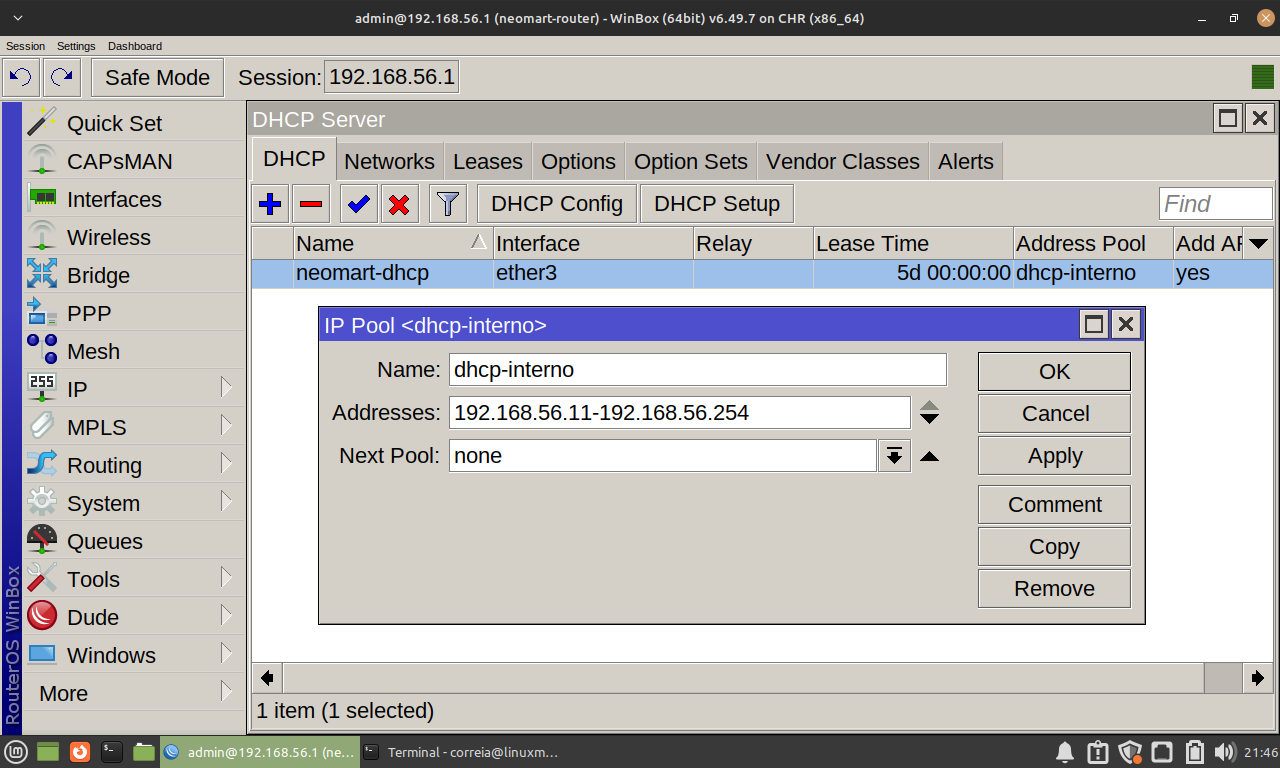
\includegraphics[height=0.5\textwidth]{roteador-dhcp-range.png}
\caption{Configuração do DHCP}
\label{fig:dhcp}
\end{figure}

\newpage

\subsection{Firewall}
Optamos pela solução tanto de software quanto de hardware. Adequando desde das máquinas dos funcionários até os servidores e garantindo também o controle da nossa rede interna. Os seguintes softwares serão utilizados: Windows Firewall e ufw, para suprir nossas necessidades locais nas demais máquinas dos setores e inclusive o do TI. Já para a rede optamos por utilizar um dispositivo de firewall chamado Fortinet FortiGate do modelo 101F FG-101F.

\subsection{Armazenamento em Nuvem}
O armazenamento em nuvem será fornecido através do serviço Google Drive com o plano Business Standard, através de seu dashboard somos capazes de analisar, mensurar e realizar o backup a partir do servidor de arquivos.

\subsection{Hotspot}
Através de um roteador conhecido como hotspot podemos disponibilizar a rede WI-FI apenas para os usuários que realizarem o check-in no Facebook, ou que ao conectar, forneça um método de cadastro onde o usuário deve informar o seu endereço de E-mail por exemplo, e logo após isso, liberar a internet.\newline
Utilizaremos no projeto um roteador da Intelbras do modelo Hotspot 300, ele fornece uma interface de comunicação onde o usuário deve, para poder ter acesso a Internet, realizar o check-in na página do supermercado NeoMart no Facebook.

\section{Sistema de Gestão}
Utilizaremos o sistema ERP da empresa Bluesoft, disponibilizado pela companhia NeoMart em todas as máquinas dos funcionários da rede. Este software possibilitará:

\begin{enumerate}
    \item Gerenciamento de preços, estoque e promoções;
    \item Gestão de etiquetas de preço e balanças;
    \item Controle de fluxo de caixa e contas a pagar e receber;
    \item Gestão de bens do empreendimento;
    \item Controle e gestão de pessoas através do cadastro de funcionários;
    \item Controle logístico.
\end{enumerate}

\begin{figure}[ht]
\centering

\includegraphics[height=0.2\textwidth]{Logo-bluesoft.png}
\caption{Logo da Empresa Bluesoft}
\label{fig:adds-pastas}
\end{figure}

\section{Endereçamento IP}
Para a segurança e um maior controle sobre os computadores do setores, criamos a seguinte rede: 192.168.56.0/26, onde o Gateway possuirá o serviço DHCP operando no endereço 192.168.56.1/26.

\subsection{Detalhes Sobre a Rede}
São fornecidos 62 IP(s) para os hosts dentro de 4 sub-redes, totalizando 248 hosts válidos. Todos os computadores e outras máquinas internas ficaram disposta na primeira sub-rede, indo de 192.168.56.2 até 192.168.56.62, dentro dos IP(s) disponibilizados na primeira sub rede, 10 deles serão exclusivos para os computadores com os servidores internos do setor de TI e as impressoras, este range de IP não serão controlados pelo DHCP, nas seguintes faixas exibimos o layout do endereçamento (primeira sub-rede):

\begin{center}
\begin{tabular}{| l | r | r | r | r |}
\hline 
Setores & Faixas & Utilizados & Disponíveis & Modo\\
\hline
Servidores & .1/26 - .10/26 & 2 & 60 & Estático\\
PC(s) TI e Impressoras & .1/26 - .10/26 & 6 & 54 & Estático\\
Caixas & .11/26 - .62/26 & 15 & 36 & Dinâmico\\
BackOffice & .11/26 - .62/26 & 15 & 21 & Dinâmico\\
SAC & .11/26 - .62/26 & 8 & 13 & Dinâmico\\
\hline
\end{tabular}
\end{center}

\subsection{Detalhes adicionais}
Dentro da primeira sub-rede, 13 IP(s) estarão disponíveis para os demais dispositivos externos.

\section{Estrutura da Rede}

\subsection{Cabeamento}
A rede cabeada que utilizaremos é com base na comunicação Fast Ethernet podendo alcançar até 100 Mbps em taxa de transferência dos dados. Os provedores de Internet escolhidos, juntamente com a seleção dos equipamentos ativos da rede, garantiram a disponibilidade e a baixa latência da conexão durante o horário de pico do supermercado. Utilizaremos na instalação do cabeamento par-trançado do tipo CAT-6 com espessura máxima de 915 metros, que interliga-rá todos os equipamentos ativos da rede, dos computadores as impressoras, cada setor possuirá um switch que interliga-rá as máquinas, os switch(s) por sua vez iram se conectar-se ao switch “central” do setor de TI, onde poderemos manipular e controlar cada setor com uma faixa de IP(s) fornecida pelo serviço DHCP instalado.
.
\subsection{Estratégica de RAID}
Utilizaremos a estratégia tecnológica do RAID 10 com 4 (quatro) discos rígidos de 1Tb cada, a tecnologia consiste em fragmentar as informações dividindo-as sobre os dois discos rígidos que por sua vez irão através do módulo controlador, replicar sua informações para outros 2 discos mantendo-o sempre atualizados e possibilitando uma possível recuperação local dos dados dos demais discos. Em caso de danos de mais de 2 (dois) discos, será necessário realizar uma recuperação a partir do armazenamento em nuvem pelo Google Drive.

\begin{figure}[ht]
\centering
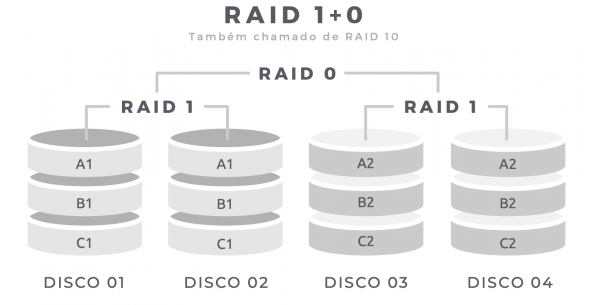
\includegraphics[height=0.3\textwidth]{RAID10.png}
\caption{Configuração de RAID}
\label{fig:adds-pastas}
\end{figure}

\subsection{Redundância e Disponibilidade Dentro da Rede}

\subsubsection{Links e Provedores}
Utilizaremos com o propósito de garantir a disponibilidade da rede e o rápido suporte aos possíveis problemas de conexão, 2 (dois) links de internet através de dois provedores diferentes, que são eles: Planalto Net e Piernet, ambos localizados em Carpina-PE com boas recomendações, o preço dos links estão dispostos no orçamento de rede do projeto.

\subsection{Segurança Física e Redundância nos Servidores}
Optamos por utilizar um sistema de ponto, onde a partir dele obteremos o controle e o log dos funcionários do setor de TI, por meio dele poderemos ter o controle do acesso físico as máquinas especializadas em controlar as demais dentro da empresa. No que se trata da redundância nos servidores, utilizaremos componentes adicionais, que são eles HD(s): 8x4TB; Pente de Memórias: 8x8GB. Estes componentes adicionais ficaram guardados em um local estocável de forma segura para uma possível substituição no futuro se caso algum problema ocorrer. Disponibilizamos de um Nobreak que possui 4 portas, sendo duas delas ocupadas pelos servidores, fornecendo a proteção elétrica, garantindo o isolamento e evitando quedas ou desligamento acidental da fonte de energia.

\subsection{Memória Adicionais}
Para uma rápida manutenção corretiva, incluímos diversos pentes e discos de armazenamento adicionais, para que haja um estoque rápido de componentes para agilizar a correção de problemas corriqueiros dentro do servidor.

\subsubsection{Nobreak}
Para evitar picos e quedas de energia, um Nobreak será instalado nos servidores, garantindo a não interrupção e a não corrupção dos documentos que ainda não foram feitos o backup, ou que ainda estão em espera pelo procedimento. Mantendo o coração da rede vivo, podemos nos preocupar com a elaboração das medidas aprofundadas para os demais computadores da rede.

\subsection{Políticas de Segurança da Informação (PSI)}
As políticas de segurança estão voltadas a ampla utilização das máquinas e dos servidores dispostos na rede, os funcionários devem seguir as políticas dentro dos seus respectivos setores, o objectivo central das políticas é de estabelecer padrões de condutas para desde a utilização virtual através do uso de software a utilização físicas, desde da adaptação e separação dos componentes envolvidos.

\begin{center}
\begin{tabular}{| l | r | r | r |}
\hline 
ID da Política & Políticas\\
\hline
1 & Criação de Senhas\\
2 & Trocas de Senhas\\
3 & Armazenamento de Senhas\\
4 & Níveis de Acesso\\
5 & Uso dos Computadores\\
6 & Encriptação de Dados\\
7 & Prevenção Contra Ransomware\\
\hline
\end{tabular}
\end{center}

\subsection{Detalhes das políticas de segurança}

\subsubsection{Criação de Senhas}
Criação de Senhas: Cada usuário terá que redefinir sua senha, que deverá respeitar o seguinte padrão: Cada senha deverá conter com no mínimo 12 carácteres sendo eles formador por; números; letras maiúsculas e minúsculas; carácteres especiais (@ \# \$ \& \_), o usuário também terá limitações nos horários de entrada e de saída e ficará a critério da empresa decidir os horários.

\subsubsection{Troca de Senhas}
Troca de senhas: Os funcionários devem trocar suas senhas dentro de 60 dias (2 meses). Além disso, o funcionário não pode reutilizar as 10 últimas senhas previamente utilizadas em seu usuário.

\subsubsection{Armazenamento de Senhas}
As credenciais de acesso de todos os funcionários serão armazenadas
no sistema do ADDS e numa cópia física mantida em um local seguro, de modo em que apenas as pessoas autorizadas terão acesso, com isso elas estarão livres de eventuais perdas de dados já envolvendo a questão do não repúdio.

\subsubsection{Níveis de Acesso}
Cada grupo de funcionários terá seu nível de privilégio dentro do sistema limitando também o acesso deles a rede interna. Políticas como essas dão a possibilidade de gerenciar os dados produzidos pelos mesmos em sua máquina local gerenciando também o desempenho de cada funcionário, proporcionando também uma forma viável de realizar o controle das informações que trafegam por elas.

\subsubsection{Encriptação de Dados}
Os dados internos como os de faturamentos, indicadores e contratos com parceiros por exemplo serão criptografados para uma maior segurança antes de serem enviados para o Google Drive, com isso garantimos a segurança com a confiabilidade e disponibilidade dos dados produzidos e distribuídos para a internet.

\subsubsection{Uso dos Computadores}
Os usuários deverão respeitar as condutas de uso dos computadores, que são elas: Não plugar dispositivos de armazenamento, como: Pendrive, Cartão de Memória e HD(s)/SSD(s) na máquina; Ao sair da máquina, bloquear-la para evitar possíveis ataques físicos de terceiros à máquina; Reportar potenciais problemas tantos de Software quanto de Hardware ao funcionários do setor de TI.

\subsection{Plano de Contingência}
Nos dias atuais, se tornou um grande problema algo conhecido como RaaS (Ransomware as a Service) ou Ransomware como serviço, é um tipo de malware extremamente danoso para as empresas e organizações, pois os criminosos que realizam este tipo de ataque tem por objetivo criptografar as informações que são demasiadamente importantes para as empresas e cobrar um ou mais resgates pela mesma, e o maior problema é que o mecanismo de segurança quebrada que possibilita este tipo de invasão é feita de dentro da empresa, por algum funcionário mal intencionado que deseja através do ataque, extorquir a empresa com a ajuda dos atacantes, para se proteger é extremamente importante ter um backup adequado e controlar a entrada e o controle de acesso aos servidores internos de maneira extremamente efetiva.

\subsubsection{Prevenção de Ransomware}
Utilizando uma estrutura simples e ao mesmo tempo confiável de Backup e Antivírus com o gerenciamento de nível de acesso, irão possibilitar uma proteção rígida contra eventuais ataques de Ransomware que possam vir do mau uso dos computadores pelos funcionários.Evitando assim possíveis vazamentos ou roubo de dados.

\section{Topologia Final}
Propusermos a seguinte configuração para o ambiente físico: Dois provedores de Internet recendo dois links de 100MB interligando-o ao roteador principal do setor de TI, saindo com a conexão da rede privada (LAN) para o dispositivo de Firewall da Fortinet, esse por sua vez ligando ao Switch central do setor de TI, e o switch central aos demais setores! Os setores de BackOffice e SAC dispõem de dois pontos de acesso (um pra cada) para a comunicação entre Notebooks e/ou tablets.

\section{Virtualização}
A virtualização é um método criado para fornecer máquinas virtuais, ou seja, que rodam em modo software sobre uma máquina hospedeira. Uma solução adequada ao mercado é a implantação do serviço hipervisor Proxmox. O Proxmox é gratuito e de código aberto, e por rodar em um sistema GNU/Linux nos garante a confiabilidade e disponibilidade do serviço e a partir dele podemos construir nosso ambiente da maneira mais adequada e estruturada possível (mostrada nos benefícios do ambiente virtual).

\begin{enumerate}
    \item É gratuito (Livre e de código aberto).
    \item Ajustável ao esquema de RAID 10.
    \item Sendo um hipervisor (Fornece abstrações de sistemas de arquivos, endereços MAC entre outros).
    \item Altamente responsivo (Permite o administrador gerenciar e visualizar o uso dos recursos como CPU, RAM e Armazenamento).
    \item Sistema completo de Backup das máquinas.
    \item Gerenciamento das máquinas através da rede.
\end{enumerate}

\subsection{Benefícios da Virtualização}
A partir da virtualização podemos construir um ambiente de testes chamado também de homologação, onde podemos testar novas configurações antes de implantar no ambiente produtivo, no neǵocio em si. Tudo isso resultará em um ambiente rápido e produtivo. Os principais benefícios são:

\begin{enumerate}
    \item Reduzir custos na compra de Hardware.
    \item Diminuir o tempo de implementação.
    \item Reusar e distribuir recursos do servidor.
    \item Manter os ambientes reais seguros.
    \item Consolidar projetos.
\end{enumerate}

\section{Plano de Backups}
Estabelecer um plano de backup eficiente visando reter de maneira eficiente e de forma incremental os dados gerados pelas máquinas dos setores dispostos tanto dentro quanto fora da empresa, nós propomos as seguintes divisões sobre o plano de Backups para possibilitar sua realização sem transtornos adicionais ou imprevistos, esses são: Esquematização dos Backups; Política de Backups; Materiais Necessários; Serviços Necessários.

\subsection{Esquematização dos Backups}
Para uma boa lógica de backup, é de extrema necessidade propor a estratégia utilizada para ir desde da escolha à realização do backup dentro de um ambiente corporativo. Itens como: Modelo de Backup; Periodicidade; Prioridade dos Dados; Criptografia Utilizada no Backup.

\subsection{Políticas de Backup}
Estabelecemos essas políticas com base nas necessidades dentro do setor do supermercado, com o objetivo de elucidar as normas e o meio para a realizar o backup de modo eficiente e seguro.

\begin{center}
\begin{tabular}{| l | r | r | r |}
\hline 
Id da Política & Política & Modo de Backup\\
\hline
1 & Modelo do Backup & Incremental\\
2 & Periodicidade & Diariamente\\
3 & Prioridade dos Dados & Documentos e Dados do Sistema\\
4 & Criptografia Utilizada & Simétrica (Cloud também)\\
\hline
\end{tabular}
\end{center}

\subsubsection{Modelo de Backup}
Propomos a utilização do modelo incremental, neste modelo de backup é necessário um backup completo das máquinas 1 (uma) vez na semana, após isso, no dia a dia, somente os dados que foram gerados ou editados irão ser salvos encima da duplicação dos dados criados no dia anterior, com exceção ao do Backup Total; aumentando assim a eficiência no quesito de velocidade e do consumo de banda no que cabe às máquinas dos setores.

\subsubsection{Periodicidade}
Será realizado diariamente através de um software o backup sem que haja a necessidade de intervenção, o mesmo fará tal backup com cerca de 3H de antecedência antes de começar o expediente, para que assim não haja interferência na demanda do dia a dia. 

\subsubsection{Prioridade dos Dados}
É necessário estipular com os demais setores os dados que são de importância para os setores em questão, nem todo tipo de informações criadas pelos funcionários são de importância para o funcionamento da empresa, levando em consideração a não necessidade dos mesmos de possuírem um backup com ou sem versionamento dentro dos servidores corporativos. Ademais, alertar sobre o uso do servidor de arquivos é de extrema importância para os dados considerados importantes para empresa aos funcionários.

\subsubsection{Criptografia Utilizada nos Backups}
Utilizaremos o já mencionado software VeraCrypt numa partição virtual de no mínimo 1TB, estabelecendo uma partição criptografada com \textbf{"AES SHA 512"} sobre a mesma senha do servidor ADDS (para fins didáticos).

\subsection{Materiais Necessários}
Utilizaremos o software chamado “\textbf{Cobian Backup}” para realizar a nossa esquematização de backup de forma automática, 1 (uma) vez dentro da semana o software realizará um Backup Total e ao longo da semana, backups incrementais. Para concretizar o backup é de extrema importância possuirmos espaço extra para realizar os backups totais e incrementais, e sempre tentando armazená-los pelo maior tempo possível e de novo, o Cobian nos ajudará a manter esta proposta. Para a criptografia utilizaremos o já mencionando VeraCrypt.

\section{Confidencialidade das Informações}
Os funcionário deverão assinar um termo de confidencialidade juntamente ao seu contrato de trabalho, na qual esteja explícito a política do não vazamento das informações transitada dentro do ambiente de negócios da empresa, ações como (fotos; gravações), caso o funcionário acabe vazando tais dados, ele poderá ser altamente prejudicado, com até mesmo sua própria demissão, ou em casos ainda mais graves, responder judicialmente.

\section{Orçamentos}

\subsection{Softwares}

\begin{center}
\begin{tabular}{| l | r | r | r | r |}
\hline 
Software & Quantidade & Licenciamento & Valor Unitário (R\$) & Valor Total (R\$)\\
\hline
Norton Small Business & 2 & 2 Anos & 766,00 R\$ & 1.532,00 R\$\\
Debian Server & 1 & Vitalício & - & Gratuito\\
Windows 10 Pro & 38 & Vitalício & 819,00 R\$ & 31.122,00 R\$\\
Server 2019 Essentials & 1 & Vitalício & 2.989,00 R\$ & 2.989,00 R\$\\
Office 365 Enterprises & 38 & Mensal & 76,80 R\$ & 2.918,40 R\$\\
CCleaner & 38 & Vitalício & - & Gratuito\\
NordVPN Complete & 1 & 2 Anos & 1.719,90 R\$ & 1.719,90 R\$\\
VeraCrypt & 1 & Vitalício & - & Gratuito\\
Cobian Backup & 38 & Vitalício & - & Gratuito\\
Proxmox & 1 & Vitalício & - & Gratuito\\
Squid & 1 & Vitalício  & - & Gratuito\\
nginx & 1 & Vitalício & - & Gratuito\\
bind9 & 1 & Vitalício & - & Gratuito\\
\hline
\end{tabular}
\end{center}
\subsection{Recursos e Serviços de Rede}
\begin{center}
\begin{tabular}{| l | r | r | r |}
\hline
Hardwares e Serviços & Quantidade & Valor Unitário & Valor Total\\
\hline
Planalto Net Link de Internet & 1 & 149,00 R\$ & 149,00 R\$\\
Piernet Link de Internet & 1 & 125,00 R\$ & 125,00 R\$\\
Rolo de Cabo - CAT-6 (~300 metros) & 3 & 469,00 R\$ & 1.407,00 R\$\\
Conector RJ-45 - CAT6 (100 un.) & 3 & 29,38 R\$ & 88,14 R\$\\
\hline
\end{tabular}
\end{center}

\subsection{Hardwares}
\begin{center}
\begin{tabular}{| l | r | r | r | r |}
\hline 
Hardware & Quantidade & Valor Unitário & Valor Total & Referenciado\\
\hline
Computadores Desktop & 38 & 2.777,59 R\$ & 105.548,42 R\$ & KaBuM!\\
Notebook & 2 & 3.059,10 R\$ & 6.118,20 R\$ & Extra\\
Servidores & 2 & 6.199,99 R\$ & 12.399,98 R\$ & KaBuM!\\
HD 4TB (Redundância) & 8 & 449,99 R\$ & 3.599,92 R\$ & KaBuM!\\
Memória RAM (Redundância) & 8 & 199,99 R\$ & 1.599,92 R\$ & KaBuM!\\
Impressoras \& Monocromática & 4 & 2.199,99 R\$ & 8.799,96 R\$ & KaBuM!\\
Nobreak \& (Para os servidores) & 3 & 389,99 R\$ & 1.169,97 R\$ & KaBuM!\\
Relógio de Ponto & 2 & 219,90 R\$ & 439,80 R\$ & Magazine Luiza\\ 
Impressora Térmica & 15 & 179,03 R\$ & 2.685,45 R\$ & Magazine Luiza\\
Leitor de Código de Barras & 15 & 97,89 R\$ & 1.468,35 R\$ & Magazine Luiza\\
Roteador MikroTik & 1 & 1.527,65 R\$ & 1.527,65 R\$ & KaBuM!\\
Switch & 4 & 755,10 R\$ & 3.020,40 R\$ & KaBuM!\\
Ponto de Acesso & 1 & 159,13 R\$ & 318,26 R\$ & Americanas\\
Roteador Hotspot & 1 & 160,55 R\$ & 160,55 R\$ & Nagem\\
Leitor de Fitas & 1 & 3.327,00 R\$ & 3.327,00 R\$ & Dell\\
Dispositivo de Firewall & 1 & 35.000,00 R\$ & 35.000,00 R\$ & Americanas\\
\hline
\end{tabular}
\end{center}

\subsection{Justificativa do Porque Optamos Pelos Principais Hardwares}

\subsubsection{Computadores Desktop}
Optamos por essas configurações para fornecer uma performance aceitável na realização das tarefas nos setores e por possuir compatibilidade com as atualizações futuras do sistema operacional, visando sempre o custo benefício:

\begin{enumerate}
    \item Processador: Intel Core I3 10100F (Frequência 3.60 GHz à 4.30 GHz) de 64 bits
    \item Memória RAM: 8GB DDR4 (Dual Channel)
    \item Armazenamento: SSD 480GB
    \item Monitor com HDMI de 21.5 polegadas (incluso)
    \item Quant. porta RJ-45 para rede: 1
    \item Adicionais: Mouse, teclado e cabo VGA inclusos
\end{enumerate}

\subsubsection{Servidores}
Os servidores escolhidos serão utilizados para controlar os usuário e fornecer os diversos serviços dentro da empresa, por causa da demanda e da necessidade de prover serviços como o ADDS, optamos por servidores de alto desempenho que compõem as seguintes características:

\begin{enumerate}
    \item Marca: Lenovo
    \item Modelo: ST50
    \item Processador: Intel Xeon E-2224G 4C - Frequência: 3.5GHz
    \item Memória RAM: 8GB (Tipo: TruDDR4 UDIMM - Frequência: 2666 MHz)
    \item Armazenamento 1TB (Expansível até 4 discos de 4TB 7200RPM TA III)
    \item Rede: 1x Gigabit (somente 1000) LAN OnBoard
    \item Controladora RAID: On board RAID 121i (0/1/10/5)
    \item Fonte - Potência: 250 Watts
\end{enumerate}

\subsubsection{MikroTik}
O roteador utilizado é do modelo Routerboard RB3011IIAS-TM L5, escolhido por possuir a potência necessária para a rede. Características do produto:

\begin{enumerate}
    \item Marcar e Modelo: Mikrotik Routerboard (RB3011UiAS-RM)
    \item Qnt. Portas USB: 2 (3.0 tipo A)
    \item CPU: IPQ-8064 (ARM 32bit) Quant. Núcleos: 2 - Frequência: 1,4 GHz
    \item Tamanho da RAM: 1GB
    \item Temperatura suportada: -20°C até 70°C
    \item Portas: Ethernet 10/100/1000 - Quant. 10 - Tipo: RJ45
\end{enumerate}

\subsubsection{Switch}
O dispositivo utilizado é da TP-link, modelo Tl-sg1024 ao qual possui 24 portas RJ-45 com compatibilidade para interfaces de até 1Gbps, pode ser montando em racks e possui uma taxa de transferência de até 35.7Mbps, perfeito para suprir nossa demanda e possíveis melhorias nos setores no longo prazo, como aumentar a quantidade de máquinas.

\subsubsection{Pontos de Acesso}
O AP selecionado possui as seguintes características:

\begin{enumerate}
    \item Marcar e Modelo: Intelbras AP360
    \item Banda suportada: Até 300Mbps
    \item Potência de transmissão de 630mW (400m2)
    \item Tecnologia Qualcomm: estabilidade e qualidade do sinal
    \item Adicionais: WI-FI de um fabricante líder em WI-FI \& Exclusivo dispositivo de segurança contra furto!
\end{enumerate}

\subsubsection{Ponto Biométrico}
Optamos por escolher um dispositivo conhecido como "Ponto Biométrico" que registrará as entradas e saídas em referência aos dois servidores físicos da rede. O propósito é garantir a maior segurança visando a disponibilidade e integridade dos servidores e ao próprio não-repúdio.

\subsubsection{Hotspot}
O dispositivo foi escolhido com o foco na plasticidade e confortabilidade, já que o requisito para acessar a internet é feito através da realização do check-in no Facebook, uma tarefa prática e fácil além da configuração do roteador ser bastante facilitada pelo próprio sistema da Intelbras.

\subsubsection{Leitor de Fitas}
O leitor optado suporta até 12TB da capacidade básica e pode chegar a 30TB no modo de capacidade comprimida.

\subsection{Orçamento Total}
\begin{center}
\begin{tabular}{| l | r | r | r |}
\hline 
Divisão do orçamento & Orçamento Total\\
\hline
Softwares & 40.281,30 R\$\\
Recursos e Serviços de Redes & 1.769,14 R\$\\
Hardwares & 187.183,83 R\$\\
Mão de Obra (30\%) & 68.770,28 R\$\\
Valor Total do Projeto & 298.004,51 R\$\\
\hline
\end{tabular}
\end{center}

\section{Referencias}
\bibliographystyle{sbc}
\bibliography{sbc-template}

Disponível em: <\url{https://www.magazineluiza.com.br/access-point-wireless-300mbps-ap360-intelbras-cx-1-un/p/jd4be13c8d/rc/rcnm/?&seller_id=infotechti}>. Acesso em: 27 set. 2022.

Disponível em: <\url{https://www.kabum.com.br/produto/129456/switch-tp-link-tl-sg1024d-utp-frame-jumbo-10kb-24-portas}>. Acesso em: 27 set. 2022.
Disponível em: <\url{https://www.magazineluiza.com.br/leitor-codigo-de-barras-com-febraban-laser-usb-lcb-180-exbom/p/bh26jj2b8k/pi/lcbr/}>. Acesso em: 27 set. 2022.

Disponível em: <\url{https://www.kabum.com.br/produto/259227/routerboard-MikroTik-rb3011iias-tm-l5-padrao-ethernet}>. Acesso em: 29 nov. 2022.

Disponível em: <\url{https://www.magazineluiza.com.br/mini-impressora-portatil-bluetooth-termica-58mm-android-ios/p/dg062c918a/in/ipst/?&seller_id=megaecommerce&utm_source=bing&utm_medium=pla&partner_id=69009&msclkid=8aaf090475281b80238a6a2a7f390596}>. Acesso em: 27 set. 2022.

Disponível em: <\url{https://www.kabum.com.br/produto/104472/impressora-epson-workforce-m5299-jato-de-tinta-monocromatica-wi-fi-bivolt-m5299?gclid=Cj0KCQjwsrWZBhC4ARIsAGGUJuq_PsGzIOpJCx7KoDGkIT7LmDSrYEZsicRKVoiq7IzqlzzKQjfJqCYaArd-EALw_wcB}>. Acesso em: 27 set. 2022.

Disponível em: <\url{https://www.magazineluiza.com.br/microsoft-windows-10-professional-fqc-09478/p/ab6b3ab72j/in/sowa/}>. Acesso em: 27 set. 2022.
Getting Debian. Disponível em: <\url{https://www.debian.org/distrib/}>. Acesso em: 12 out. 2022.

Piernet telecom. Disponível em: <\url{http://www8.piernet.com.br/plano/black/}>. Acesso em: 12 out. 2022.

PlanaltoNET Sta. Cruz do Rio Pardo. Disponível em: <\url{https://www.planaltonetsantacruz.com.br/}>. Acesso em: 12 out. 2022.

Disponível em:
<\url{https://www.kabum.com.br/produto/170108/microsoft-windows-server-2019-essentials-64-bits-coem-midia-fisica-g3s-01294?srsltid=AR5OiO16qkLTj4dDTt1grODDe0F3TF5U0-tOiRllAtvzyNRNCDUXgbMHcY8}>. Acesso em: 29 set. 2022.

Disponível em: <\url{https://nordcheckout.com/pt-br/payment/?product_group=nordvpn&currency=BRL&bundle_type=complete&step2_nav_off=true&cart_id=2258f51e-bc84-471c-a615-de5fc0d663e3}>. Acesso em: 5 out. 2022.

Disponível em: <\url{https://www.microsoft.com/pt-br/microsoft-365/enterprise/compare-office-365-plans}>. Acesso em: 5 out. 2022.

Disponível em: <\url{https://www.kabum.com.br/produto/132024/servidor-lenovo-thinksystem-st50-xeon-e-2224g-4c-71w-3-5ghz-8gb-1tb-7y481002br?srsltid=AR5OiO3hbbgOVjUHZaQ0aVmWT_jpyqxxy4K14aLd3AYx90Rsq3g6Ua_Rg7I}>. Acesso em: 5 out. 2022.

Disponível em: <\url{https://www.kabum.com.br/produto/89940/memoria-corsair-vengeance-lpx-8gb-2666mhz-ddr4-c16-preto-cmk8gx4m1a2666c16}>. Acesso em: 5 out. 2022.

Disponível em: <\url{https://www.kabum.com.br/produto/95803/hd-seagate-4tb-barracuda-3-5-sata-st4000dm004}>. Acesso em: 5 out. 2022.

squid: Optimising Web Delivery. Disponível em: <\url{http://www.squid-cache.org/}>. Acesso em: 26 out. 2022.

Rolo De Cabo De Rede Cat6 Preto - 305 M - Mk2 Tecno. Disponível em: <\url{https://produto.mercadolivre.com.br/MLB-1332224273-rolo-de-cabo-de-rede-cat6-preto-305-m-mk2-tecno-_JM}>. Acesso em: 26 out. 2022.

COBIAN, L. CobianSoft - the home of Cobian backup. Disponível em: <\url{https://www.cobiansoft.com/cobianbackup.html}>. Acesso em: 8 nov. 2022.

Disponível em: <\url{https://www.kabum.com.br/produto/271174/nobreak-intelbras-attiv-600va-semi-senoidal-120v-4-tomadas-de-saida-preto-4822200?srsltid=AYJSbAcOON_U_UCSFKOENvwX4UbC0fFAZGMCgNuQj8oBlLpEBAXyTs5s2os}>. Acesso em: 8 nov. 2022.

Proxmox - Powerful open-source server solutions. Disponível em: <\url{https://www.proxmox.com/en/}>. Acesso em: 9 nov. 2022.

NAGEM. Roteador Intelbras Wireless 300Mbps HotSpot-300, Informática - NAGEM. Disponível em:
<\url{https://www.nagem.com.br/produto/detalhes/473197/Roteador+Intelbras+Wireless+300Mbps+HotSpot-300}>. Acesso em: 9 nov. 2022.

Disponível em: <\url{https://razor.com.br/wp-content/uploads/2020/02/Screen-Shot-2020-02-03-at-14.56.46-600x305.png}>. Acesso em: 18 nov. 2022.

LTO8 de fita Media, Pacote com 1, kit de cliente | Dell Brasil. Disponível em: <\url{https://www.dell.com/pt-br/shop/lto8-de-fita-media-pacote-com-1-kit-de-cliente/apd/440-bbiu/armazenamento-e-drives}>. Acesso em: 22 nov. 2022.

Small Business. Disponível em: <\url{https://br.norton.com/products/small-business}>. Acesso em: 22 nov. 2022.

INTERNET SYSTEMS CONSORTIUM. BIND 9. Disponível em: <\url{https://www.isc.org/bind/}>. Acesso em: 29 nov. 2022.

nginx news. Disponível em: <\url{https://nginx.org/}>. Acesso em: 29 nov. 2022.

VeraCrypt - Free Open source disk encryption with strong security for the Paranoid. Disponível em: <\url{https://www.veracrypt.fr/code/VeraCrypt/}>. Acesso em: 22 nov. 2022.

Disponível em: <\url{https://razor.com.br/wp-content/uploads/2020/02/Screen-Shot-2020-02-03-at-14.56.46-600x305.png}>. Acesso em: 22 nov. 2022a.

Disponível em: <\url{https://www.americanas.com.br/produto/5070308588?opn=YSMESP&offerId=627bb89a87c00289c211510b&srsltid=AYJSbAe6Fa9SdE0FRxRFbVHhFb3n0REGGZvThXw6f29UiQlYOp1AYLkVzcQ}>. Acesso em: 22 nov. 2022b.

Disponível em: <\url{https://www.kabum.com.br/produto/269569/conector-RJ45-cat6-fortrek-pacote-com-100un?srsltid=AYJSbAcmv-J-HdXprhtq4I6SHn-9ec99uxbnNwmfwCQjXsv8ficbr24LrK0}>. Acesso em: 30 nov. 2022b

Disponível em: <\url{https://www.kabum.com.br/produto/190834/computador-completo-facil-intel-core-i3-10100f-decima-geracao-8gb-ddr4-geforce-ssd-480gb-monitor-21-5-hdmi?srsltid=AYJSbAeRnTi4i9e9IA4gsAwFH1dItgmJBK4_6DRF8Jdai6CRJOLze-ruDpY}>. Acesso em: 1 dez. 2022.

Relógio de Ponto. Disponível em: <\url{https://www.magazineluiza.com.br/relogio-de-ponto-biometrico-digital-control-id-eletronico-kp-1028-knup/p/ak61eafh58/pi/atrp/}>. Acesso em: 1 dez. 2022.

BLUESOFT. Bluesoft ERP - Sistema ERP Cloud - Verdadeiramente na Nuvem. Disponível em: <\url{https://bluesoft.com.br/}>. Acesso em: 1 dez. 2022.

\newpage

\section{Apêndice 1}

\subsection{Credenciais de Acesso as Máquinas do Ambiente Virtual}

\begin{enumerate}
   \item Debian Web: mart\#\$03500u
   \item Debian Samba: neo56429518!cogito
   \item Debian DNS: 45genterinside@
   \item Windows Server: ordered\$QUIT5294
   \item Windows Cliente: susuki69@barroNei
   \item Linux Mint Cliente: 528520QSC\$\$uv
   \item Roteador: rockonyou12@97892
\end{enumerate}

\newpage

\section{Apêndice 2}

\begin{figure}[ht]
    \centering
    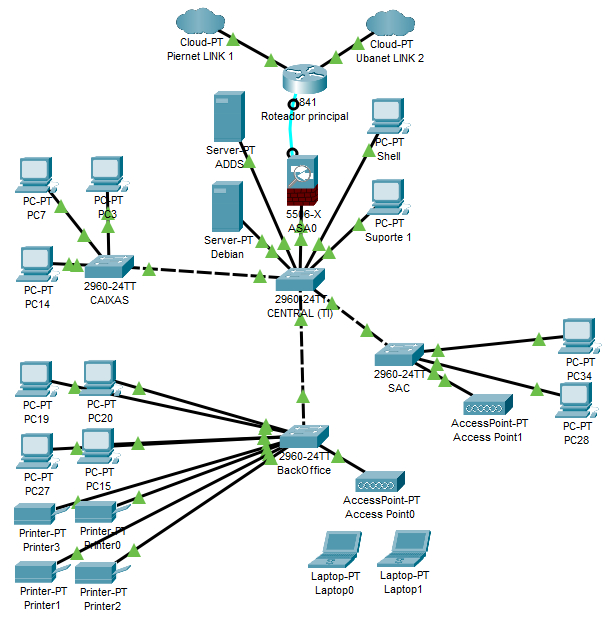
\includegraphics[height=0.7\textwidth]{cisco01.jpeg}
    \caption{Topologia aplicada}
    \label{fig:cisco-topologia}
\end{figure}

\newpage

\section{Apêndice 3} 

\begin{figure}[ht]
    \centering
    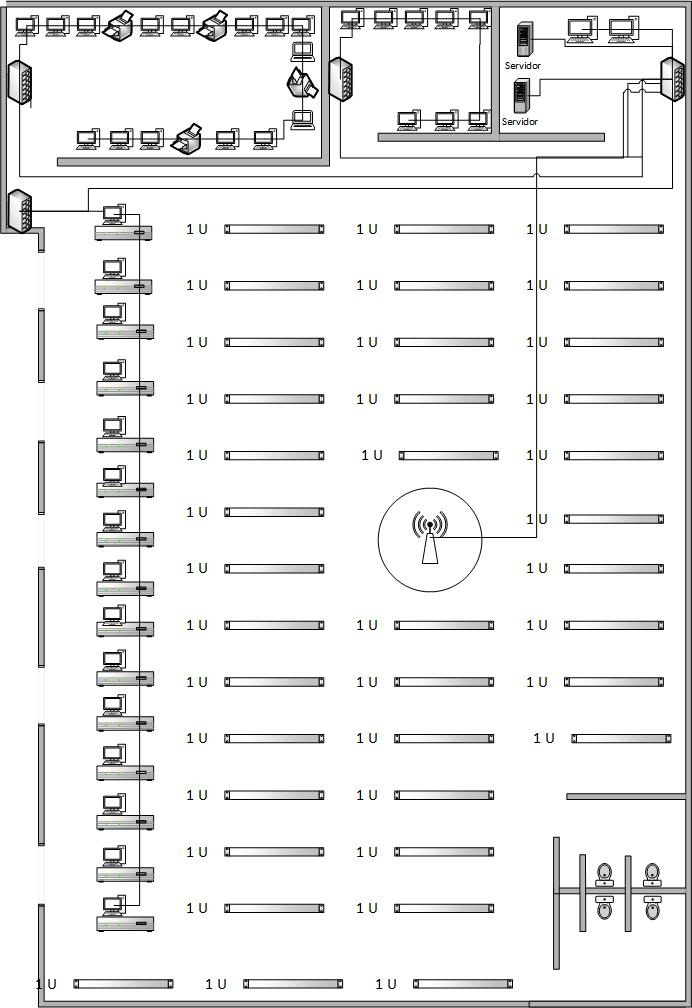
\includegraphics[height=0.7\textwidth]{planta PI II.jpg}
    \caption{Planta da NeoMart}
    \label{fig:cisco-topologia}
\end{figure}

\newpage

\section{Apêndice 4}

\subsection{Termo de Confidencialidade e de Uso das Máquinas}

\begin{verbatim}
                                __/__/__ CARPINE-PE NeoMart
\end{verbatim}

Comprometo-me através das minhas atribuições alto declarar ciente e vi-emente aos seguintes termos de conduta com relação ao trafego de informações dentro e fora da empresa NeoMart. O termo em questão pode e deve ser usado somente se um ou mais dos critérios não forem obedecidos. Os critérios também são aplicáveis aos funcionários ao qual sofreram exoneração de seus cargos e que possam possuir de algum meio que por vias de intimidação ou suborno vier a prejudicar a empresa. 

\begin{enumerate}
    \item Utilizar uma senha de forma que não seja necessária uma recuperação prévia no ato de realizar o login, como o de escrever em um papel perecível ou que possa comprometer a integridade da sua máquina e da rede interna.
    \item Acessar as máquinas somente em horário empresarial.
    \item Bloquear a máquina quando não presente, garantindo a segurança física da sua própria máquina.
    \item Respeitar as devidas regras aplicadas ao seu ambiente virtual e inclusive ao ambiente físico.
    \item Salvar todos os arquivos no que se refere a empresa - ARQUIVOS PESSOAIS NÃO SÃO PERMITIDOS - no servidor de arquivos que está disposto para o usuário em sua área de trabalho.
    \item Comprometer a não violação das políticas de segurança (PSI) e em caso de exoneração, está ciente das atribuições legais realizadas através da assinatura desse contrato.
\end{enumerate}

O funcionário(a) que de algum modo violar um dos critérios estabelecidos poderá ser indiciado e exonerado de seu cargo e/ou forçado a prestar esclarecimentos sobre o artificio legal da irresponsabilidade na quebra do termo proposto.
\newline
\newline
\begin{verbatim}
    ________________________        ________________________
       Nome do Funcionário              Nome do Gerente
\end{verbatim}

\newpage

\section{Apêndice 5}

\subsection{Termo de responsabilidade na administração da rede}

\begin{verbatim}
                                __/__/__ CARPINE-PE NeoMart
\end{verbatim}

Eu funcionário da NeoMart do setor da Tecnologia da Informação, TI, através desse artificio legal, declaro consciente e complacente e disposto a seguir e da responsabilidade no manuseio e configuração dos elementos de redes incluindo os computadores; servidores; e demais ativos de redes dentro e fora da empresa NeoMart por meio da utilização do serviço de conexão remota, os seguintes termos:

\begin{enumerate}
    \item Realizar a manutenção preventiva e corretiva caso necessário.
    \item Realizar o cópia do backup para o servidor de arquivos na nuvem e para as fitas, essa por sua vez utilizando-se do leitor previamente instalado no setor de tecnologia.
    \item Aplicar e configurar os dispositivos ativos de redes em seus setores.
    \item Garantir a não interrupção completa dos setores envolvidos dentro da empresa em horário de trabalho.
    \item Garantir o comprimento do termo de responsabilidade.
\end{enumerate}
    
\begin{verbatim}
    ________________________        ________________________
      Nome do Funcionário              Nome da Coordenação
\end{verbatim}

\end{document}
